
\documentclass[a4paper, oneside, 11pt]{report}
\usepackage{epsfig,pifont,float,multirow,amsmath,amssymb}
\newcommand{\mc}{\multicolumn{1}{c|}}
\newcommand{\mb}{\mathbf}
\newcommand{\mi}{\mathit}
\newcommand{\oa}{\overrightarrow}
\newcommand{\bs}{\boldsymbol}
\newcommand{\ra}{\rightarrow}
\newcommand{\la}{\leftarrow}
\usepackage{algorithm}
\usepackage{algorithmic}
\usepackage{natbib}
\topmargin = 0pt
\voffset = -80pt
\oddsidemargin = 15pt
\textwidth = 425pt
\textheight = 750pt

\begin{document}

\begin{titlepage}
\begin{center}
\rule{12cm}{1mm} \\
\vspace{1cm}
{\large  CMP-7009A Advanced Programming Concepts and Techniques}
\vspace{7.5cm}
\\{\Large Project Report - 16 January 2020}
\vspace{1.5cm}
\\{\LARGE Simulating the activities of an Ant colony}
\vspace{1.0cm}
\\{\Large Group members: \\ Alvin Lu}
\vspace{10.0cm}
\\{\large School of Computing Sciences, University of East Anglia}
\\ \rule{12cm}{0.5mm}
\\ \hspace{8.5cm} {\large Version 1.0}
\end{center}
\end{titlepage}


\setcounter{page}{1}
%\pagenumbering{roman}
%\newpage


\begin{abstract}
An abstract is a brief summary (maximum 250 words) of your entire project. It should cover your objectives, your methodology used, how you implemented the methodology for your specific results and what your final results are, your final outcome or deliverable and conclusion. You do not cover literature reviews or background in an abstract nor should you use abbreviations or acronyms. In the remainder of the report the chapter titles are suggestions and can be changed (or you can add more chapters if you wish to do so). This template is designed to help you write a clear report but you are welcome to modify it (at your peril ...). Finally, a guideline in size is approximately 3,500 words (not including abstract, captions and references) but no real limit on figures, tables, etc.
\end{abstract}

\chapter{Introduction}
\label{chap:intro}

The biological world has always been a source of inspiration for computer models and algorithms. Within successful model developed, swarm intelligence have always been a topic of interest spanning across wide range of disciplines \citep{Swarm_Intro}. In computing, swarms are usually associated with ants that exhibits large amount of behaviours that can potentially be used to optimise algorithms. Whilst there exist techniques and simulations \citep{Ant_Simulator} \citep{Ant_Simulator_Revisited} \citep{Ant_Simulator_Intro}  that mimics the certain behaviour of ants, there aren't software available that simulate ants realistically in  the biological world.

This project aims to develop a realistic ant simulator that allows customisation of various biological settings to simulate different ant colonies in varying environments. It will provide a method to show an accurate representation of ant behaviours, simulate survivability or ants in different settings, and reveal emergent properties that may benefit future swarm intelligence.


\section{MoSCoW}
\subsection{Must}
\begin{tabular}{|| p{3.5cm} | p{10.5cm} ||} 
	\hline
	Requirements & Description \\
	\hline
	Independent ant movements & Ants must move independently from each other \\
	\hline
	Creating hive & Allow creation of a hive. The hive will be the starting point of all ants belonging to that hive. \\
	\hline
	Static food & Allow creation of static food items on the map. \\
	\hline
	Pheromone types & Contain a pheromone system that allows deposition of pheromone values on the ground. \\
	\hline
	Pheromone evaporation & Deposited pheromones should decrease in concentration overtime in a fixed rate. \\
	\hline
	Obstacle creation & Able to create obstacles that ants can't move on or under \\
	\hline
	Ant births & Able to dynamically generate ants in with a given birth rate \\
	\hline
	Ant death & Ants will die and be removed from the map by probabilistic death rate \\
	\hline
	Pause and play simulation & Allow users to pause the running simulation and replay it multiple times \\
	\hline
	Shows ant data dynamically & Shows ant population and time elapsed on the UI dynamically  \\
	\hline
\end{tabular}

\subsection{Should}
\begin{tabular}{||p{3.5cm} | p{10.5cm} ||} 
	\hline
	Requirements & Description \\
	\hline
	Customisable hive location & The hive location of ants should be customisable on allowed locations on the map. \\
	\hline
	Customisable food location & Food items should be customisable on allowed locations on the map. \\
	\hline
	Customisable global evaporation rate & Rate of evaporation of pheromones can be customised\\
	\hline
	Reset simulation & Allows resetting the simulation with different values \\
	\hline
	Time scaling & Automatically scales the time to reflect realistic values. Allow users to enter actual values for attributes that are connected to time.\\
	\hline
\end{tabular}

\subsection{Could}
\begin{tabular}{|| p{3.5cm} | p{10.5cm} ||} 
	\hline
	Requirements & Description \\
	\hline
	Multiple hives & Allows creation of multiple ant colonies with varying population \\
	\hline
	Customizable terrain & Terrains can be customised by the users by painting pixels on the map \\
	\hline
	Moving food item & Allows creation of food item that moves across the screen \\
	\hline
	Predator & Allows creation of predators that attacks and consumes the ants\\
	\hline
	Customisable individual evaporation rate & Allows customisation of individual evaporation rates \\
	\hline
	Preset ant settings & Provides a list of settings that reflects actual values of ant species \\
	\hline
	Varying ant types & Allows creation of different types of ant within a colony \\
	\hline
	Pheromone data at point & Outputs the pheromone data of a particular point in the map\\
	\hline
	Creation of new pheromones & Allows creation of pheromones with different properties\\
	\hline
\end{tabular}

\subsection{Won't}
\begin{tabular}{|| p{3.5cm} | p{10.5cm} ||} 
	\hline
	Requirements & Description \\
	\hline
	Detailed UI models &  The UI of different items(sprites) in the simulator will not have detailed models and will be represented by simple shapes\\
	\hline
	In-built screen recording & The system will not provide recording features \\
	\hline
	Nupital flight simulation & The system will not simulate the process of nupital flight \\
	\hline
\end{tabular}

\section{Report structure}
Breifly describe what you will cover in the remainder of the report, chapter by chapter.

\chapter{Background}
\section{Motivation}
Swarming is a behaviour that is commonly found in social animal species \citep{Swarm_Animals}. The concept of swarming is having a large group of individually operating unit (agents or individual animal) working together to achieve a task that is typically to great for a unit to complete on its own \citep{Swarm_Explanation}. Large amount of research has been conducted to explain the evolutionary benefits of such behaviour and researchers are aiming to adapt some of these properties into various computer systems. This is commonly achieved by having a group relatively simpler agents that can communicate between each other instead of a singular system to complete tasks collectively by converging individual accomplishments \citep{Swarm_Properties}.

Within animals that exhibit swarming, ants are one of the insect that has been vigorously studied for their behaviour. Ants most commonly utilise swarming during the process of foraging. Certain species of ants are shown to leave pheromones to share information an individual ant has learnt \citep{Ant_Pheromones}. The two most common pheromones are home pheromones that can guide them home and also pheromones that guide other ants to food sources \citep{Ant_Pheromones}. 


\section{Existing research and methods}
Currently, an ant simulator was found publicly available online that uses the MASON simulation toolkit \citep{Mason}.

\begin{figure}[htb]
	%\begin{center}
	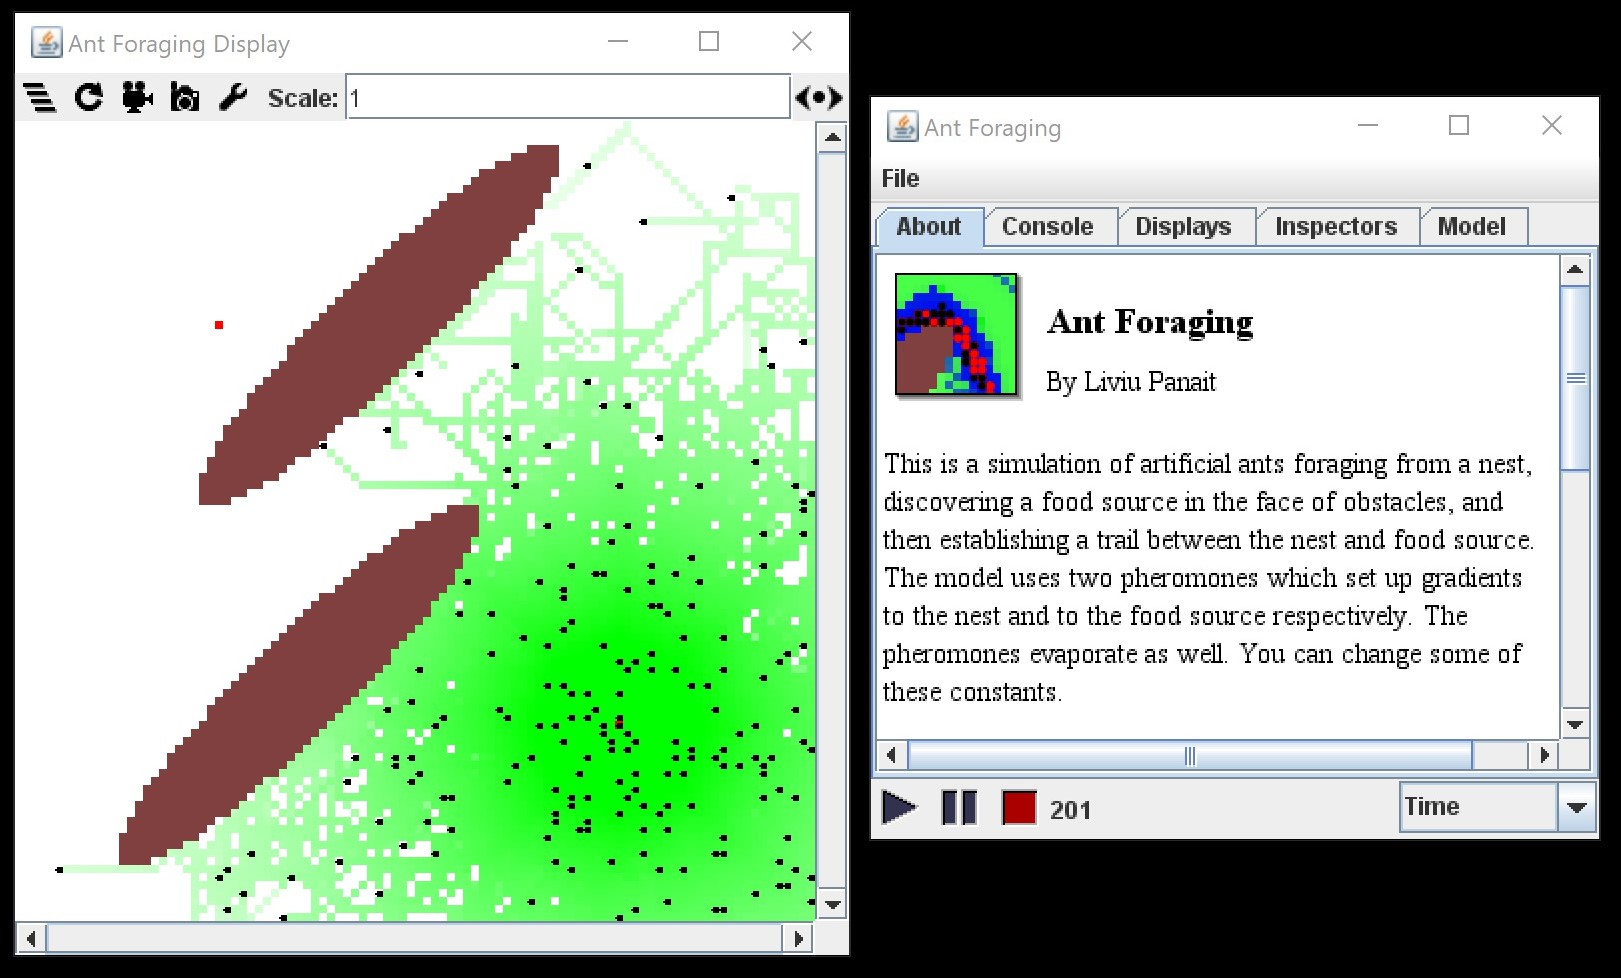
\includegraphics[width=1.0 \columnwidth]{MASON_Ant.jpg}
	\caption{Ant simulator developed by Liviu Panait}
	\label{MASON_Ant}
	%\end{center}
\end{figure}

\chapter{Methodology}

Describe here various methods that will be used in your project. Use different sections for distinctly different subjects and use subsections for specific details on the same subject. Only use subsubsections or paragraphs (which are not numbered) if you believe this is really necessary. 

\section{Method 1}
\subsection{Method 1 specific detail 1}
In case you need maths, here is an example to write an equation:
\begin{equation}\label{weak_form}
\int_{\Omega_0} \delta u \frac{\partial \mathbf{P}}{\partial X}d\Omega_0 + \int_{\Omega_0} \delta u \mathbf{b} d\Omega_0 + \int_{\Omega_0} \delta u  \rho_0\mathbf{\ddot u} d\Omega_0 = 0
\end{equation}
And here we show how to write a matrix equation:
\begin{equation}\label{Jacobian}
 \mathbf{X}  \frac{\partial N}{\partial e_c} =  \left[  \begin{array}{cccc} x_1 & x_2 & x_3 & x_4 \\  y_1 & y_2 & y_3 & y_4 \\  z_1 & z_2 & z_3 & z_4 \end{array} \right] \left[  \begin{array}{ccc} 1 & 0 & 0 \\ 0 & 1 & 0 \\ 0 & 0& 1 \\  -1 & -1 &  -1  \end{array} \right] 
\end{equation}


\subsection{Method 1 specific detail 2}
blablabla

\paragraph blablabla

\section{Method 2}

\subsection{Method 2 specific detail 1}

\section{Etc.}

\subsection{Etc.}

\chapter{Implementation}

In this chapter you cover the actual implementation of your project.
This is likely to require figures such as Fig.\ \ref{Pelvis_BVH}.

\begin{figure}[htb]
%\begin{center}
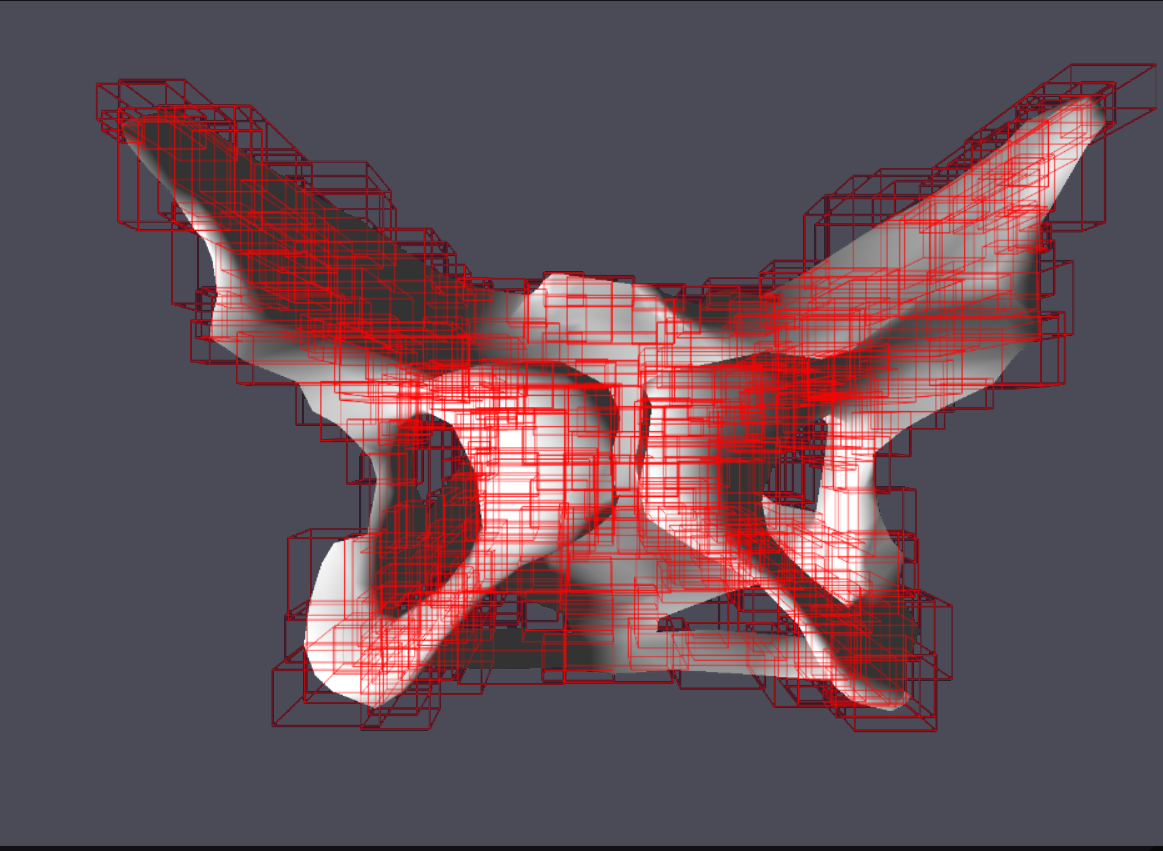
\includegraphics[width=1.0 \columnwidth]{pelvis_octree.png}
\caption{The bony pelvis model with octree based AABBs (Axis Aligned Bounding Boxes).}
\label{Pelvis_BVH}
%\end{center}
\end{figure}

Or better - a UML diagram (class, sequence and state diagrams are the preferred ones) as shown in Fig.\ \ref{class}:

\begin{figure}[htb]
%\begin{center}
\includegraphics[width=1.0 \columnwidth]{class.png}
\caption{A UML class diagram.}
\label{class}
%\end{center}
\end{figure}

Or perhaps an algorithm (if it does not belong in the Methodology chapter instead).

\begin{algorithm}[th]
\caption{ The projection based contact method algorithm }
\begin{algorithmic}[1]
\STATE Retrieve current node displacement $u$
\\ \texttt{float3 u = m\_U\_new[nodeIndex].xyz;}
\STATE Retrieve constraint plane equation
\\ \texttt{float4 plane = m\_constraintMagnitude[nodeIndex];}
\STATE Calculate dot product with plane normal
\\ \texttt{float d = dot(u, plane.xyz);}
\STATE Find node penetration into the plane's negative half-space
\\ \texttt{float penetration = plane.w - d;}
\IF {penetration is greater than zero}
	\STATE Find projection onto the plane surface
	
	\texttt{float3 proj = u + plane.xyz * penetration;}
	\STATE Prescribe new nodal position to be on the surface
	
	\texttt{m\_U\_new[nodeIndex] = (float4)(proj, 0.0f);}
\ENDIF
\end{algorithmic}
\end{algorithm}

Or perhaps a table named Table \ref{Res01} (again could be more suitable in the Methodology chapter).

\begin{table}[h]
\caption[]{Original diameters and diametral strains as reported by
  Sorbe and Dahlgren \cite{Sorbe:1983} (columns 1-2), from a previous 
  experiment by Lapeer and Prager and reported in \cite{Lapeer:2001}
  (columns 3-4), and from the current experiment (columns 5-6).}
\begin{center}
\begin{tabular}{|l|c|c||c|c||c|c|}\hline
& \multicolumn{2}{c||}{S-D} & \multicolumn{2}{c||}{L-P old} & \multicolumn{2}{c|}{L-P new} \\ \hline
Diameter & length & strain & length & strain & length & strain \\ \hline
$\mi{MaVD}$ & 140.5 & +1.90 & 129.3 & +0.30 & 129.3 & +1.43 \\
$\mi{OrOD}$ & 131.4 & +0.10 &   -   &  -    & 119.9 & +1.85 \\
$\mi{OrVD}$ & 126.9 & +2.20 & 119.3 & +0.25 & 119.3 & +1.24 \\
$\mi{OFD}$  & 134.0 & +0.40 &  -    &   -   & 119.7 & +1.82 \\ 
$\mi{SOFD}$ &  -    &   -   &  -    &   -   & 113.2 & -0.85 \\
$\mi{SOBD}$ & 117.1 & -1.70 &  88.7 & -1.07 &  88.7 & -2.52 \\
$\mi{BPD}$  & 105.0 &  0.00 &  89.7 & -0.21 &  89.7 & -0.83 \\ \hline
\end{tabular}
\label{Res01}
\end{center}
\end{table}

Note that code snippets or lists of crucial programming code or large UML diagrams should go in the Appendix/Appendices.


\chapter{Experiments (or Testing)}

Describe various experiments you designed to test your software product. In case you have protocols which cover various pages, please put them in an appendix (e.g. Appendix A).

\chapter{Results}

This chapter could be potentially merged with the previous one if testing is the only form of experiment that qualifies. Note that testing involves various levels. The ones which should definitely be done are unit tests, integration tests and user tests.

\chapter{Discussion}

Discuss the results of your software product development. This chapter could be merged with the previous one(s).

\chapter{Conclusion and Future Work}

Conclude your achievements and put them in perspective with the MoSCoW analysis you did early on. Be honest by declaring for example S categorised objectives which did not make it to the final deliverable rather than reversely modifying your MoSCoW in Chapter \ref{chap:intro}! Also discuss future developments and how you see the deliverable improving if more time could be spent. Do not put in subjective opinions or rants or excuses as to why something did not work out as planned in your report. A technical report is not a medium for complaints as there are other outlets for that typically well before you came to this stage (e.g. labs, e-mail etc.).


\bibliographystyle{unsrt}
\bibliography{References}

\chapter*{Contributions}

State here the \% contribution to the project of each individual member of the group and describe in brief what each member has done (if this corresponds to particular sections in the report then please specify these).

\chapter*{Appendix A}

Put in tables of data or protocols (e.g. for testing) or code listings or UML diagrams which may take up several pages and do not sit well in the main body text.

\end{document}

